\chapter{Considera��es Finais}\label{cpConsideracoesParciais}

No presente trabalho foi realizado o levantamento da situa��o atual do portal de algoritmos, reengenharia e modelagem. Para que seja vi�vel a evolu��o foi preciso ser feito o levantamento de requisitos, engenharia, casos de uso, diagramas relacionados e prototipa��o de telas.

Cada etapa descrita acima foi desenvolvida utilizando metodologias da engenharia de software, as interfaces gr�ficas foram desenhadas buscando o melhor caso de usabilidade, a fim de facilitar seu uso.

Algumas dificuldades foram encontradas durante o desenvolvimento do presente trabalho, como a limita��o de execu��o do portal de algoritmos em apenas um navegador de \textit{internet}. Desconhecimento das tecnologias utilizadas resultaram em um tempo maior para o entendimento de suas funcionalidades e sua arquitetura.

Para continuarmos com a evolu��o do portal de algoritmos � preciso seguir o cronograma abaixo.

\begin{enumerate}
	\item Configura��o do ambiente de desenvolvimento.
	\item Cria��o da arquitetura do portal de algoritmos.
	\item Migra��o das tabelas do banco de dados.
	\item Cria��o dos \ac{DAO}.
	\item Desenvolvimento da \ac{API} \ac{REST}.
	\item Desenvolvimento das interface gr�ficas.
	\item Configura��o do servidor de aplica��o;
	\item Implanta��o
	\item Cria��o de relat�rios.
	\item Reda��o da monografia.
\end{enumerate}

\FloatBarrier
\begin{table}[!htb]
	\centering
	\caption{Cronograma TCC 2}
	\vspace{0.5cm}
	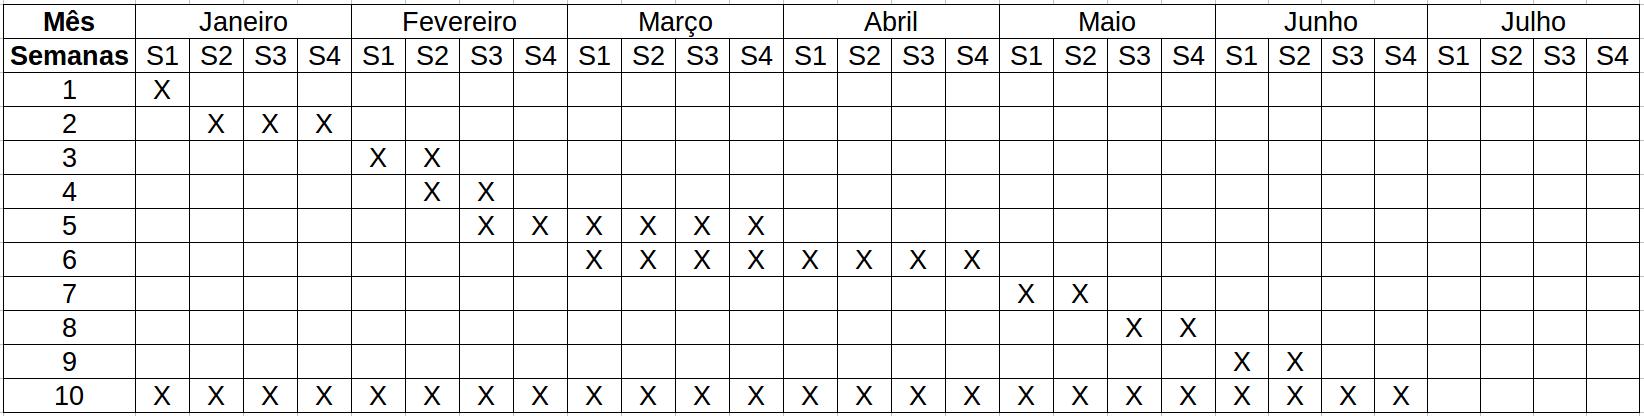
\includegraphics[width=15cm]{imagens/cronograma.png}
	\label{imgCronograma}
	Fonte (AUTOR, 2018)
\end{table}
\FloatBarrier

A figura \ref{imgCronograma} demonstra a grade do cronograma para o Trabalho de Conclus�o de Curso 2.